\documentclass[a4wide, 11pt]{article}
\usepackage{a4, fullpage}
\usepackage{graphicx}
\setlength{\parskip}{0.3cm}
\setlength{\parindent}{0cm}

% This is the preamble section where you can include extra packages etc.

% Allows licence-related quotes to be italic
\newenvironment{italicquotes}
{\begin{quote}\itshape\small}
{\end{quote}}
\begin{document}

\title{Webapps Project 2014: Final Report}

\author{Alan Vey, Octavian Tuchila, Sean Naderi}

\date{June 11, 2014}         % inserts today's date

\maketitle            % generates the title from the data above
\clearpage

\section{Introduction}
For our WebApp project, we were faced with the task of designing a program with multi-user functionality and a database maintaining some internal state. We thought the best way to go about this would be to make a website that would fulfil all of these requirements.

Given the multi-user aspect of the WebApps project, and our familiarity with version control software like Pivotal Tracker, we decided to try and make our own project management website. This seemed like a good way to meet the requirements of the project, as it encapsulates a multi-user environment as well as allowing for rich user interactions. This would also enable us to use a database to maintain internal state, as login and password information for each user would have to be stored as well as the projects that each user is part of. 

We thought that it would be useful to include different milestones for projects, with associated tasks. This way the project owner would be able to set tasks for different users to help keep the project on track and to ensure there is no overlap in tasks. These tasks could also be comment-able allowing for multi-user interaction. 

Another feature we would like to include would be an environment in which files can be edited, and different users from the same projects would be able to see this editing in real time, again adhering to the rich user interactions requirement of the project. An additional idea of ours is to allow for a messaging service to be included in this part of the website so that while editing different users can communicate with each other to discuss different aspects of the project or the current file.

All of these files and tasks would have to be stored in a database and correspond to the different users that are part of those projects or that have tasks within them, and displayed respectively for each user. This would mean that there would be a lot of internal state stored in databases which would satisfy the database requirement for this project. We plan to have certain privileges for different users corresponding to the projects owners and project participants who are added by the owner. Therefore, depending on the user, slightly different options in the page will have to be rendered to encapsulate the different user privileges; the owner is the only one who should be able to delete the project entirely, for example. 

Another element of the website that we thought would be a convenient addition is a burn down chart. A predicted finish date for the project could be derived from the cumulative difficulty assigned to each milestone in the project. This way we could plot the optimal work rate against the actual current work rate which would give the project participants a great visual way to make sure they are keeping on track.
\clearpage

\section{Project Management}
\subsection{Group Structure}
Alan was the group leader and in charge of the planning of the assignment. He also was the primary developer and so set up the project, wrote the code for all functionality of the site and sorted out all research into third party tools and deployment options. He also set up the testing infrastructure for the application.

In the beginning stages, Octavian was in charge of developing the file system to be used for the site but was met with several difficulties and so after looking into the problems, Alan realised that we could incorporate EtherPad for collaborative document editing, which handles storage itself. Thus, Octavian was assigned to the design of the entire website. 

Sean was put in charge of adding additional tests for new features and design elements. Sean used our project to plan our presentation. His feedback was useful in hashing out the small details of the site for both functionality and design.

\subsection{Implementation Language}
We decided to use the Ruby on Rails framework to develop our application. This meant between us we needed knowledge of Ruby, JavaScript/CoffeeScript, HTML and embedding, CSS and of course the Rails framework itself. Domain specific languages such as RSpec, Capybara and Factorygirl also played a role. Limited knowledge of SQL aided some debugging issues we had relating to the database.

All three of us worked on the WACC complier project together which we implemented in CoffeeScript and JavaScript giving us a solid foundation in these languages. The Ruby on Rails exercise had taught us the basics of web development so combined with the fact that none of us had any prior experience creating web based applications at least we has a good understanding of these languages. This was one of the main reasons for choosing Rails. 

We all found it really useful learning Haskell, Java and C when we first commenced our studies as these are all strongly typed languages and have a ridged development style which lead to a very solid understanding of programming. We wanted to apply the same principal to web applications by learning to develop with a framework that has a ridged set of development principals before using tools which allow for more freedom. 

Considering most of our programming knowledge is in the three languages mentioned above, we though expanding our understanding of dynamic ones would greatly benefit us making Ruby and JavaScript/CoffeeScript ideal. The process of embedding both in HTML and making use of the reflective nature of Ruby has been really interesting.

A start up Alan is working on in the summer makes use of this framework and so he was especially keen on finding out more about it. 

\subsection{Design Process}
Our division of labour lead to an efficient design process. There was no code duplication and since our responsibilities allowed for little overlap we did not have to spend much time combining the different elements. 

Initially, Alan considered using pivotal tracker to plan out our project, however this seemed to offer more functionality than required and would lead to too much complexity in setting up the project so we settled on Git, Gitlab milestones/issues and our website itself. Communication was taken care of by having regular meetings planned by Alan as well as a Facebook group chat and FaceTime. 

We used Git as a backup and collaborative development tool. Alan set up the project and got a solid foundation implemented, tested and pushed to our master branch. Alan made use of the principals of behaviour driven development for this beginning part, however given the devision of responsibility this approach was not carried on throughout the project.
From this point onwards any new functionality Alan added was done on a separate branch and merged in upon completion. 
Octavian would branch every time new functionality was added to manage the design of that part of the newly added components and merge with master when he was done. 
Sean would await the completion of functionality at which point he branched off and conducted modular testing of the models, merging back in when done and branch off again when the design was done to conduct integration testing again merging his work back to master upon completion. 

At the beginning of the project we thought of the milestones that were required and set them up on Gitlab [Figure~\ref{fig:Github}]. We subsequently added issues when they arose or we started working on a new section, assigning them to whoever we felt was best equipped to deal with them and allocating them to a milestone. This was very useful to know exactly who was working on what and making sure any problems a team member discovered were addressed by the appropriate party. 

During the feedback for our Milestone 1 review, Mark suggested we use our site to plan a part of this project. We really liked the idea and decided to plan the presentation with it writing up all supporting documentation on our collaborative real-time software. This was not only useful for the organisation of the presentation but allowed us to find minor bugs and improvements for our site. 

We usually met every two to three days to make sure the project was on track and do any of the additional tasks as well as help each other out with what we had learned. Sean would record meeting minutes and send everyone a copy on our Facebook group if required. Octavian took a keen interest in the legal aspects and helped Sean and Alan gain a better understanding after some research he had conducted. The meetings were planned using a Facebook group chat which also served as a useful tool for sharing links we found important and helping each other out with any issues we came across that we did not need to meet for.

All in all we feel this project has been a success as we have overcome many difficulties we encountered in previous tasks we completed together such as code duplication, missing deadlines, under performing and not helping each other adequately. We will definitely be planning future tasks in much more detail as we have done with this one and have all learned a lot about all the software we used to facilitate this.

\begin{figure}
  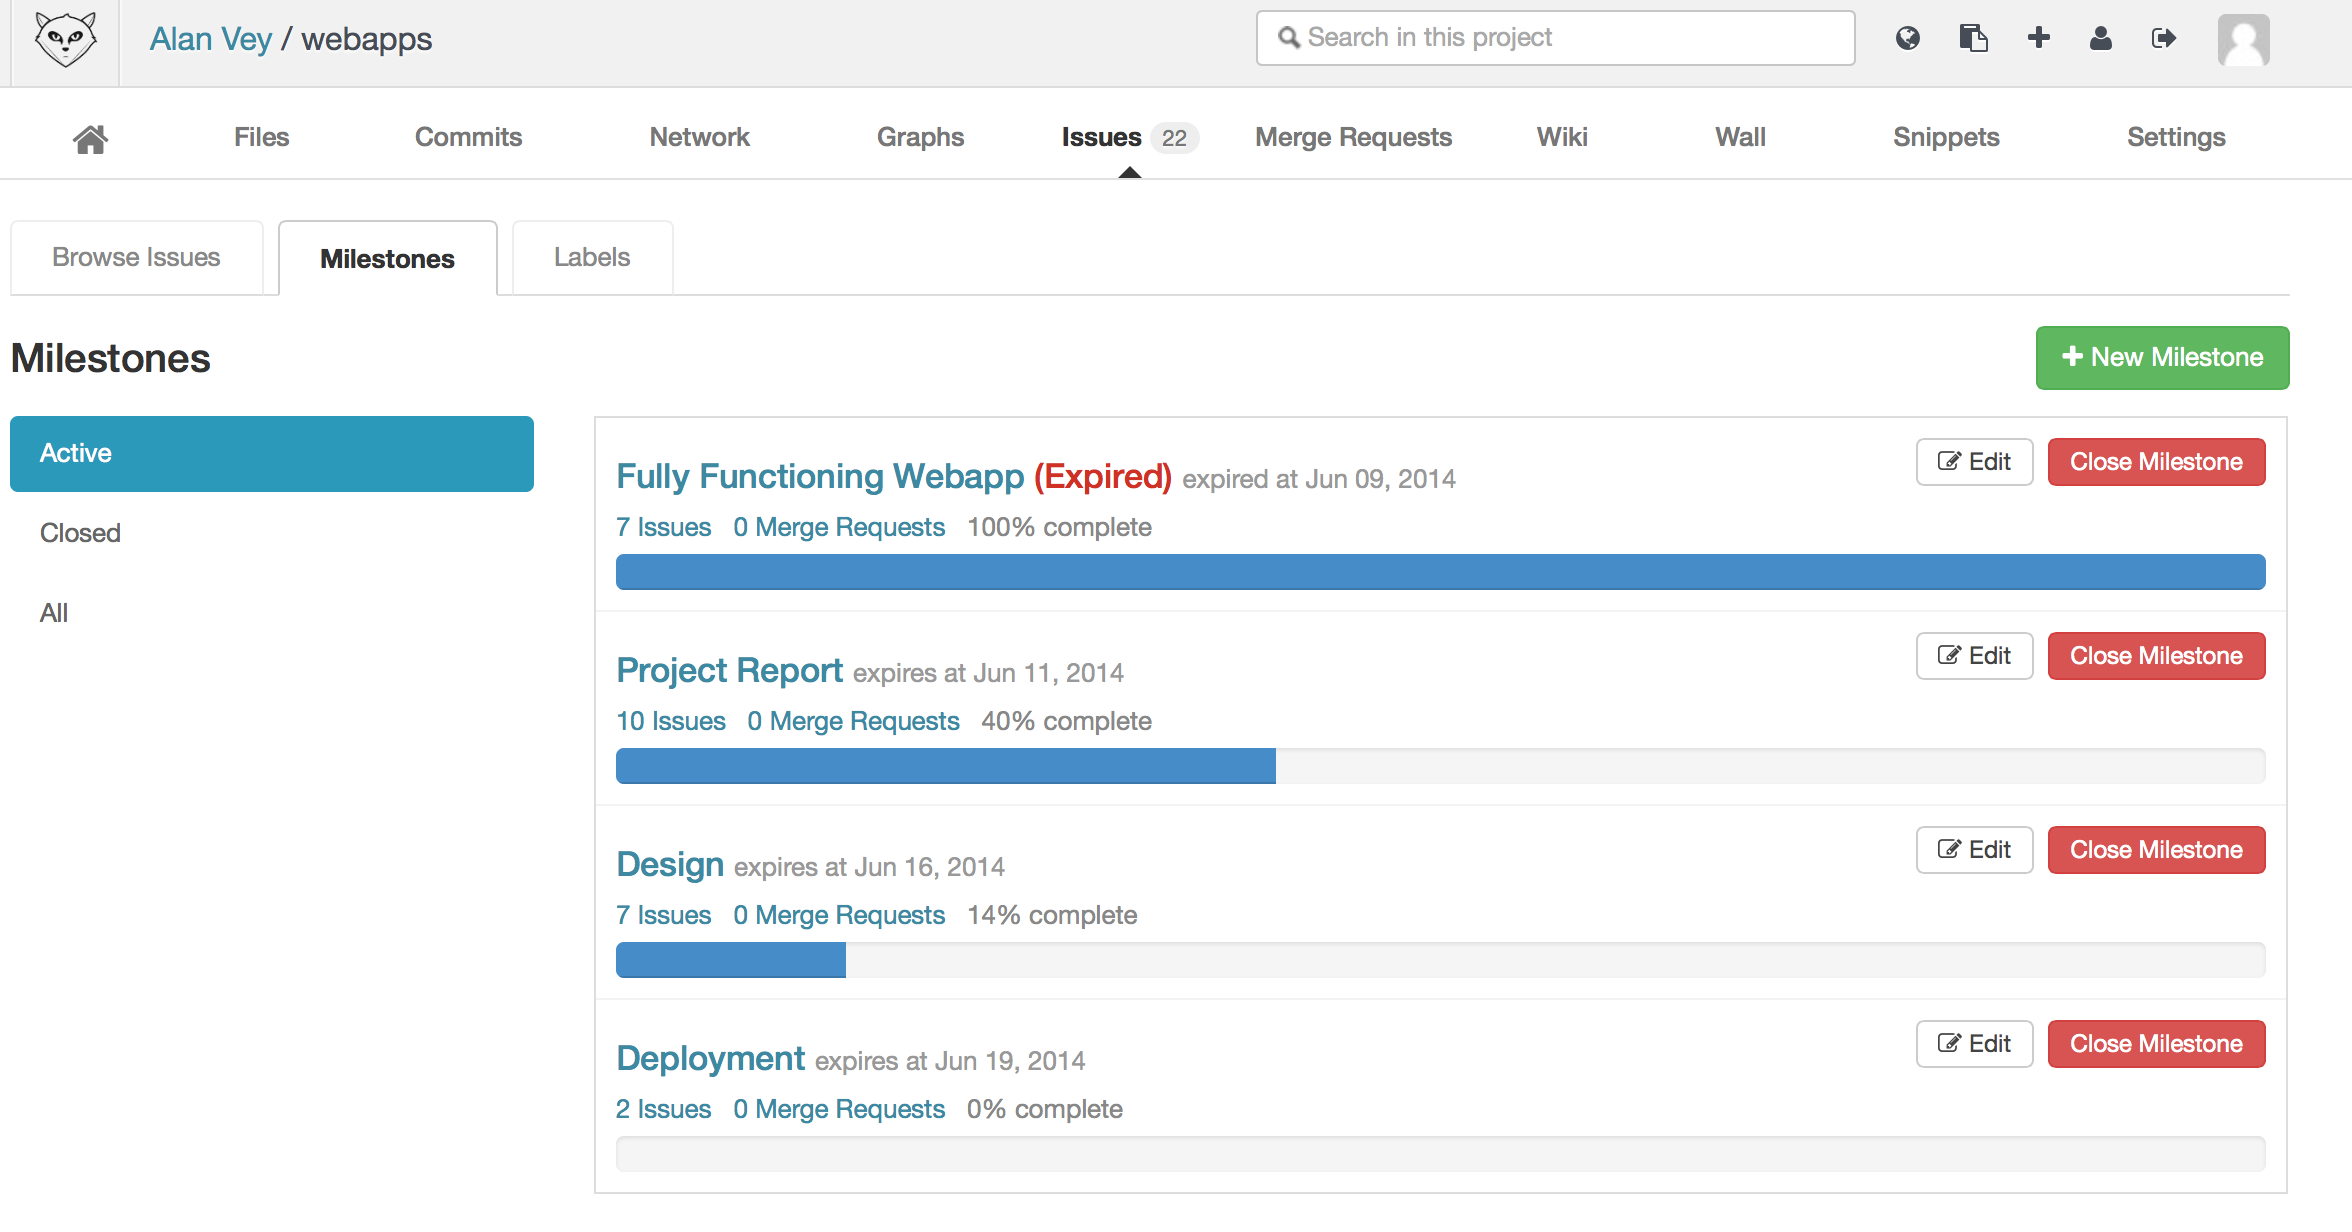
\includegraphics[width=1\textwidth]{gitlab-milestones.png}
  \caption{Overview of milestones on June 10, 2014}
  \label{fig:Github}
\end{figure}

\clearpage

\section{Program Description and Implementation Details}
\subsection{Application wide details}
Having designed our project with the Ruby (v2) on Rails (v4) framework we had to adhere to the Model-Controller-View (MVC) design pattern. We chose to place all data validation and any methods required for validation in the model classes. All of the logic for the functionality was placed in the controller classes and the views used an HTML representation of the pages with embedded Ruby and JavaScript for dynamic content. We used a PostgreSQL database because we want to deploy our application to Heroku and is thus a requirement. With very little setup, a single push to our applications master branch on Heroku has the website up and running with little configuration efforts.

\subsection{Styling and Navigation}
The styling of our website is handled mainly by the twitter bootstrap gem which some minor customisations we made to the overrides.css. 

We have a navigation bar which is fixed to the top of every page. Our site's logo is fixed to the left of the navigation bar, and this doubles up as a link to the home page so that the home page can be reached quickly from anywhere in the site. We decided to make the default page in our site the Project Listings page. The right corner has a log in button which redirects the user to the sign in page. Once signed in the navigation bar no longer has the log in button, instead it has a link with the user's email as the text, which redirects to the user account editing page. Next to that is a button to log out. This change is done with a simple authentication conditional in the layout/applications.html file.

A second navigation bar appears as soon as the user clicks on a project to navigate to that projects page. This helps easily access the project overview, management, and the editing of that project. When you click to redirect to the home page this navigation bar will disappear to show the Project Listings page. This bar is also purely generated out of bootstrap css classes and a few customisations.

\subsection{Home Page}
When navigating to our home page [Figure~\ref{fig:homepage}] at projectlab.herokuapp.com, our routing file is consulted which lists the root directory to be rendered by the home controller’s index action. This has no method body, therefore does nothing more than render the index template. The index template has a div of class .unique which loads in a background image to span the page and also renders the sign up view. From here the only other page accessible is the sign up page which has the same styling. The home page has no associated table in the database as it does not need to store anything.

\subsection{User Scaffold}
All user authentication is handled by the devise gem. We installed the devise views in order to customise the pages. When included this gem generated a users database. The only addition we made to the model was validity checks for the login email, and making sure that whenever saving an entry all fields are present. All functionality is already dealt with when it comes to creating accounts, removing accounts, updating details and encrypting saved passwords - as well as verifying input data against them. This provided some difficulty at times as one cannot edit individual controller actions, they can only be overridden.

\subsection{Project Scaffold}
The project views consist of an index, a show, an edit and a new page. The index page has a table to list projects. The new and edit pages do just as you would expect and the show page displays the project along with all of the associated project users by rendering the project users index page and a Burndown chart to display the projects status [Figure~\ref{fig:milestone}]. The project model validates the presence of the name attribute. Before routing to the index page the controller sets the projects to be listed as any that the current user owns or is a project user of. On navigating to the show page a Burndown chart is dynamically created using the googlevisualr gem, called from a class we created as the gem only supports line charts, and embedded JavaScript. The controller performs creation and deletion as one would expect.

\subsection{Project User Scaffold}
The project user scaffold is fairly simple. It has two views one for an index to list project users and one to create new project users by specifying their email. It has its model which validates an entered email address. The controller redirects any access to the index page back to the project show page, as that is where the index view is rendered. On creation, the controller verifies that the email being added is currently a user of the site, and that the project owner is not trying to add themselves as a team member. It also associates the project id with the project user on creation, as project users are nested under projects in the routing.
\clearpage

\subsection{Milestone Scaffold}
The milestone section has an index, a show, an edit and a new view. The index provides a table for the listing of milestones and the creation of new ones. The show page displays the information of the milestone, and renders the tasks index page below that. At the bottom of the page, it lists out the most recent comments associated with all the tasks belonging to that milestone. The edit and new pages do what you would expect, and are accessible from the index and show pages respectively. The milestone model validates the presence of all attributes, that the due date cannot be in the past, and that the status is one of the 4 valid options. In addition, it validates the uniqueness of the name attribute. When accessing the index page the controller sets the displayed milestones to those corresponding to the project. When the user clicks on one of them and is routed to the show page, the controller makes sure the milestone status has been updated based on the tasks. It also makes sure the tasks associated with that milestone are displayed, ordered according to priority, and the comments on all the tasks associated with that milestone are displayed ordered by recency. The create sets up the dependancies as expected as a milestone is nested under a project. 

To get to the milestone index page the user clicks on the management button on the second navigation bar. All other functionally is accessible from there.

\subsection{Task Scaffold}
The task section has an index, a show, an edit and a new view. The index provides a table that lists the tasks; along with start, finish and review buttons for each task. These conditionally appear depending on the status of the task, and whether the user is the creator of the task or the person who clicked on start. The show page displays information about that task as well as a list of comments associated with that task, and allows comments to be added. The edit and new do what you would expect and are accessible from the index and show pages respectively. The task model validates the presence of all attributes, makes sure that the associated difficulty is in the range of 1 to 10, and makes sure that the status is one of the 4 allowed strings. When trying to access the index page, the user is redirected to the milestones show page that the task is nested under. Navigating to the show page results in the controller displaying details of the task as well as all comments nested under the task. The create action sets up the nesting attributes and assigns the created status to the task. It also does some validation, and checks if the task already exists as it is not possible to validate in a model the uniqeness of two attributes. 

Tasks are assigned a difficulty estimate in days. This data is used by the Burndown chart to make estimations about a project and display the progress.
\clearpage

\subsection{Comment Scaffold}
The comments scaffold has only two views which are an index page, which lists the comments in a bootstrap formatted table, and a new page which allows the user to add a comment. The model validates the presence of all the fields before saving them to the database. In the controller, any attempt to directly access the index page is routed to the task show page as comments are nested under tasks. the create method automatically assigns the creator email and the associated task id.

\subsection{Etherpad Scaffold}
The EtherPad scaffold was generated to be the place where all files associated with a project are stored. It consists of an index, new, show and edit view. The index lists files in a table, the new allows for the creation of a new file, the edit allows changing the file name, and the show loads a file in the EtherPad software [Figure~\ref{fig:etherpad}]. This is hosted on a separate website and embedded on the show page through the use of an iFrame. The model class validates the presence of all attributes as well as the uniqueness of file and name. When accessing the index view the controller sets the files displayed in the table to be the ones associated with the project the user is currently looking at. When creating a new pad, the controller sets the project id to the current project, as Etherpads are nested under projects. It also sets the creator to the current user, and generates a random alpha-numeric string for the path so that the file is uniquely identifiable on the hosts server. 

When clicking on the edit button on the secondary navigation bar, the user is directed to the index page for the files from which all other functionality is accessible. 

\begin{figure}
  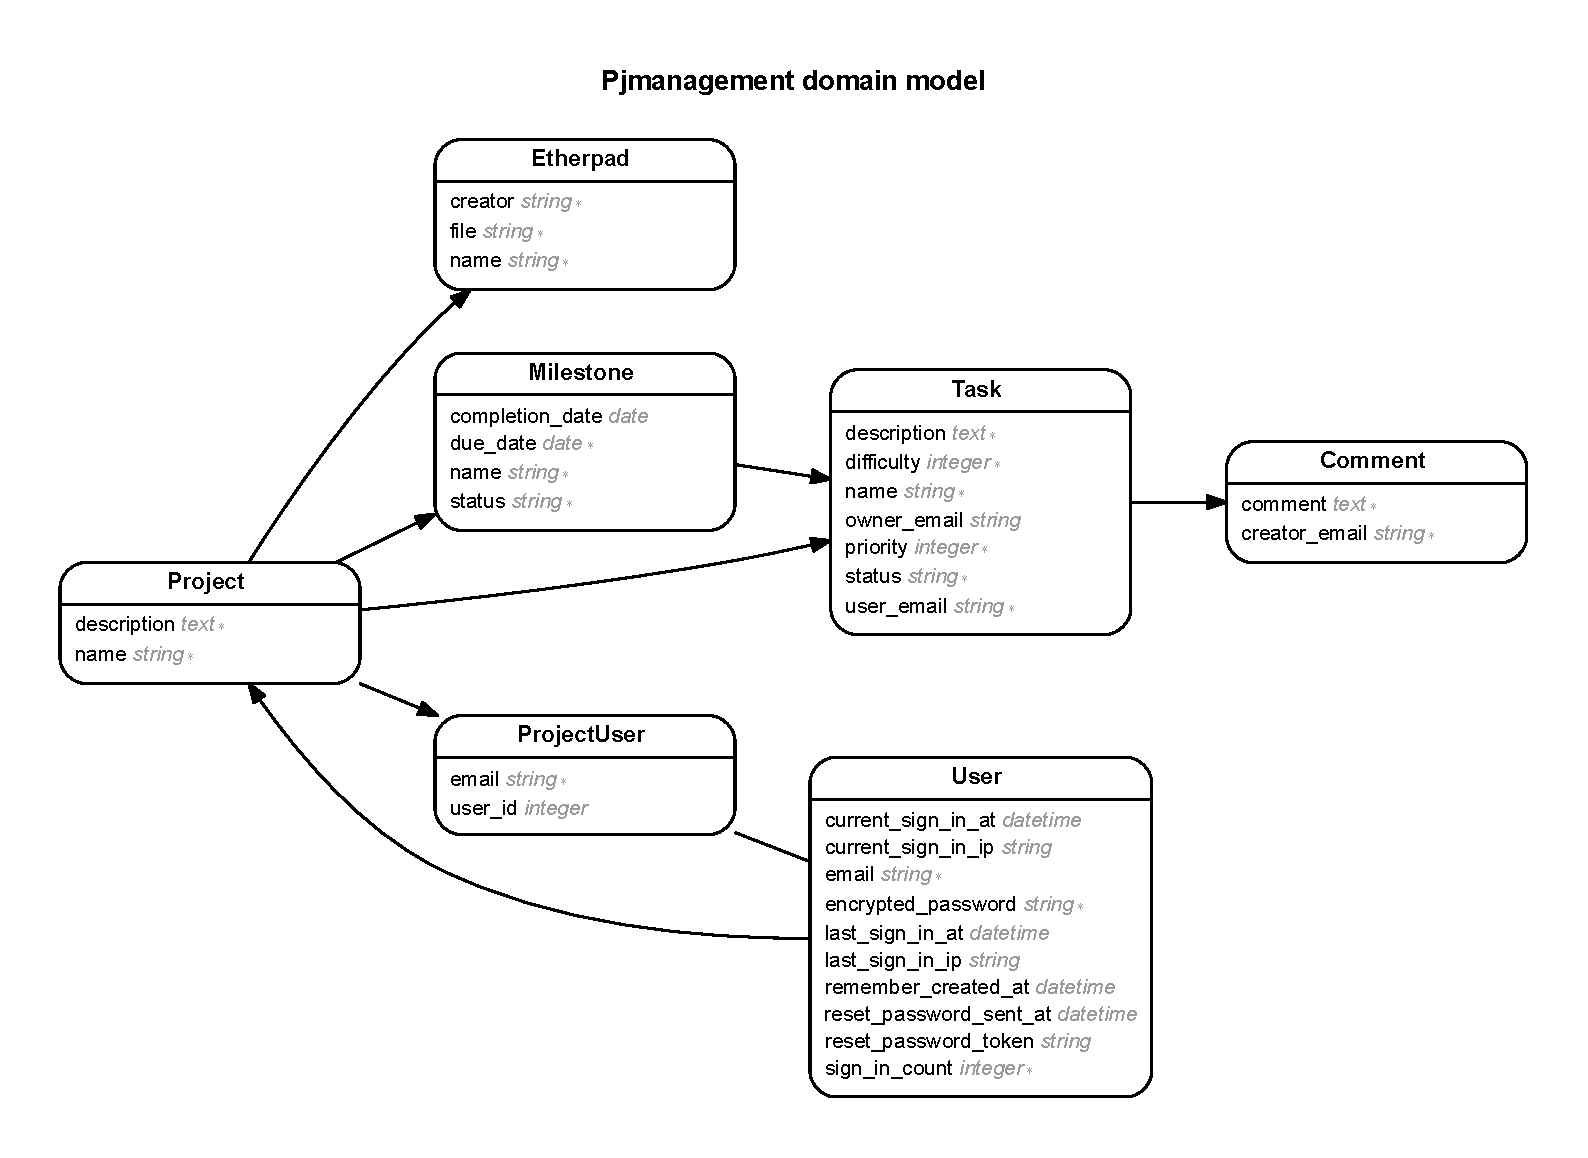
\includegraphics[width=1\textwidth]{erd.pdf}
  \caption{Database tables and relations. Note: dependants are always destroyed along with their parents in our implementation}
  \label{fig:db}

  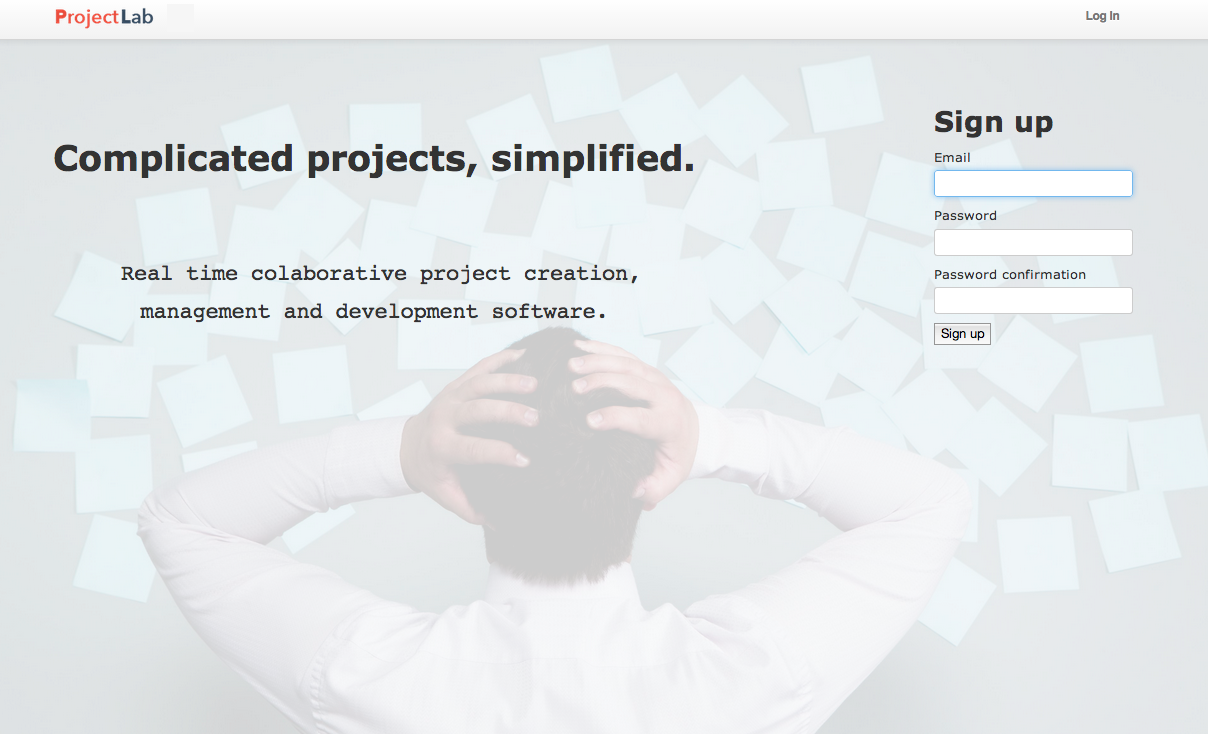
\includegraphics[width=1\textwidth]{homepage.png}
  \caption{Our homepage. Note: Styling might change slightly for the presentation}
  \label{fig:homepage}
\end{figure}}

\clearpage

\begin{figure}
  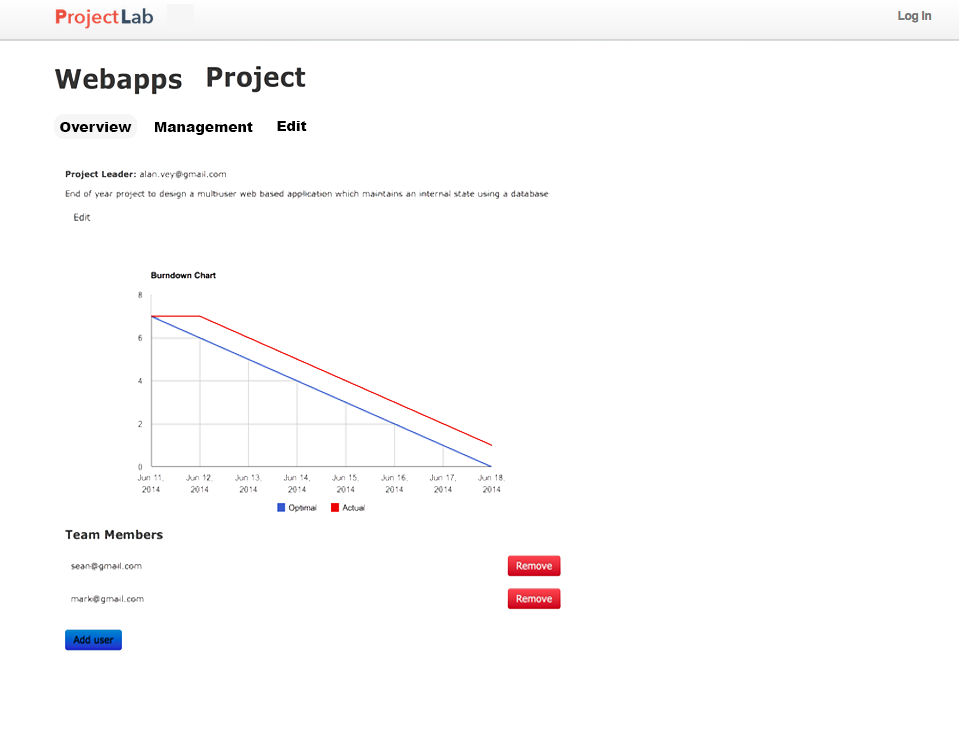
\includegraphics[width=1\textwidth]{overview.png}
  \caption{A screenshot of a project's show page}
  \label{fig:milestone}

  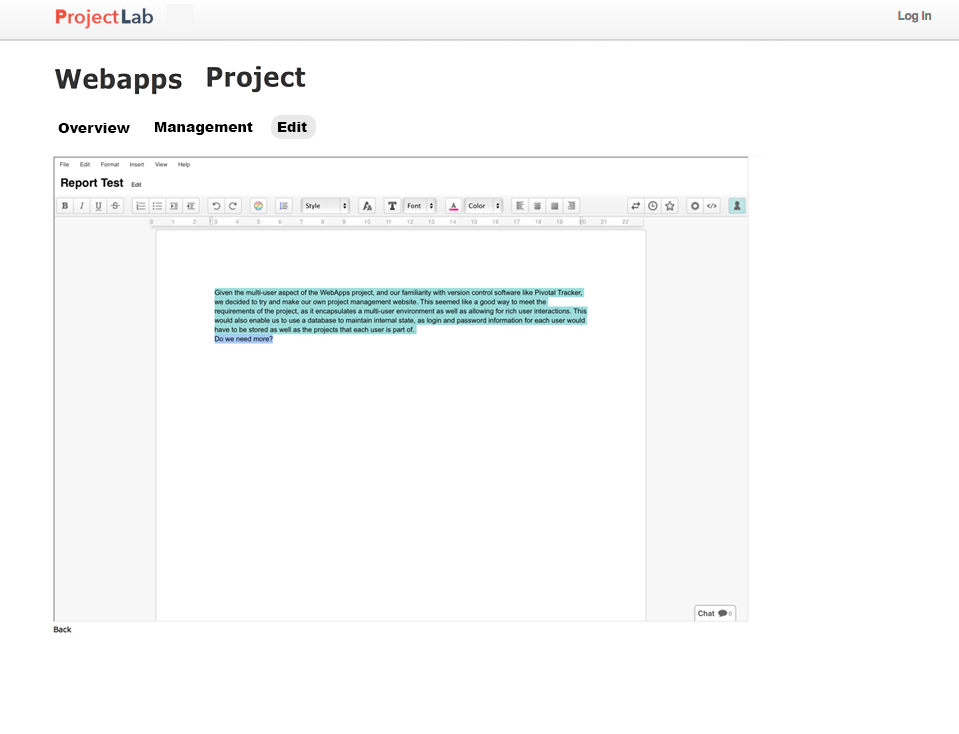
\includegraphics[width=1\textwidth]{edit.png}
  \caption{An example file opened in Etherpad, being edited by 2 users simultaneaously}
  \label{fig:etherpad}
\end{figure}}

\clearpage

\section{Legal Aspects}

We've used the Ruby programming language and its libraries, together with
several ruby gems. All these are under the Ruby Licence, which has been
accepted by the Free Software Foundation as compatible under the GPL(General
Public Licence)\cite{GNUlicence} but has not been accepted by the Open Source
Initiative. The Ruby Licence has a copyleft status, which allows copying the
code, as long as the application which is built using Ruby Licenced software is
bound by the same licence. The Ruby software has a dual licence, both under the
Ruby Licence and under the simplified BSD licence.

If we want to publish our project, we can do so under the Ruby Licence.
In order to do this, we have the following options:

\begin{italicquotes}
3. You may distribute the software in object code or binary form,
   provided that you do at least ONE of the following:

a) distribute the binaries and library files of the software,
together with instructions (in the manual page or equivalent)
on where to get the original distribution.

b) accompany the distribution with the machine-readable source of
the software.

c) give non-standard binaries non-standard names, with
instructions on where to get the original software distribution.

d) make other distribution arrangements with the author.
     \cite{Rubylicence}
\end{italicquotes}

In case we want to use the website commercially, we should act on clause 
{\it d}, by contacting the author of the Ruby programming language and the
authors of the gems we have used while building our project.

Another option for commercial distribution is to use JRuby instead of the Ruby
interpretor, as it can support Rails projects and its licence is more suitable
for commercial releases.

\begin{italicquotes}
this license is intended to facilitate the commercial use of the Program
\cite{JRubylicence}
\end{italicquotes}

We can launch our project using the following clause:

\begin{italicquotes}
a) Subject to the terms of this Agreement, each Contributor hereby grants
Recipient a non-exclusive, worldwide, royalty-free copyright license to
reproduce, prepare derivative works of, publicly display, publicly perform,
distribute and sublicense the Contribution of such Contributor, if any, and
such derivative works, in source code and object code form.
\cite{JRubylicence}
\end{italicquotes}

Furthermore, for the background, we have used a photo which we've taken off the
web. We have selected that photo specifically because the owner specified that
we are free to use it as long as we mention its origin when we place it on the
internet, within our own web application. Therefore, in case we will publish
our project, we will specify the origin of the image.

\clearpage

\section{Conclusion}

\subsection{Our project}
We have managed to successfully design a fully functional project management and real-time collaborative editing tool. We have user authentication, the functionality for project creation and a  split of every project into the categories of overview, management and editing. 

When navigating to our site one lands on the home page and can access no more until authenticated. Upon successful login the home page is no longer accessible and by default the root is set to a page listing all projects one has created or is a team member of. Clicking on any project name leads to the show page and results in a new navbar with the three categories for project design.

As the name suggests, overview gives a brief summary including the project name, description, owners email, team members and a Burndown chart to visually illustrate the progress. There is a two tier hierarchy where the project creator can edit the name and description and add team members however all other functionality is the same for any user. Obviously a project can only be accessed by the creator or a team member. 

The management page, accessible from the secondary navbar, displays a listing of milestones. Once created one can navigate to a show page for the milestone which allows for the creation of tasks and has a news feed of the most recent comments on all already created tasks. Each task can be commented on manually by navigating to their respective show pages or automatically by clicking on start and then finish and then reviewed. Again a hierarchy is used here so that only the person who started the task can finish it and only the creator of the task can review it.

The edit page contains a listing of file names and allows for the creation of additional ones. Once created, clicking on a file navigates to its respective show page which loads up the file in editing software and allows any team member working on the file to do so simultaneously, all of which is visible to ever user on the page in real-time. This software incorporates chat functionality as well as the optional download of the file. 

\subsection{Possibilities for improvement}
There are very many things we would have liked to add to our website, the main five being:
\begin{itemize}
  \item Help and supporting documentation
  \item User profiles and Private messaging
  \item Email notifications
  \item Contribution analysis
  \item Real time collaborative software for spreadsheets and presentations
  \item Gitlab integration
\end{itemize}

Supporting documentation, interactive explanations and help on the site is the most important thing missing as far as we can tell. For example whenever creating anything a small question mark would exist next to the label for the any field, which when hovered over would explain exactly what the field means and if one clicked on details would describe how it affects the project. For example creating a task; Hovering over the question mark for the difficulty would explain that this is used to keep the project on track and plays a role in the dynamic creation of the chart on the overview page. Details would redirect to the help page in a new tab, and would go into detail of the Burndown chart algorithms used.

User profiles is also a key element for improvement. Tracking the quality of users contribution as well as having some sort of team mate rating scheme and number of projects worked on would build up useful data about users which could then be used as a sort of resume when applying to work on certain projects or allow project creators to find team members with the desired skill sets. This would be modelled after websites like LinkedIn.

Email notifications are also very necessary, whether its providing updates of whats happening on projects one is part of, notification of received private messages or later notifying users of potential project prospects or suggesting team members to creators.
 
\subsection{Learning aspects}
Because Rails incorporates the basics of CSS/CSSASS, HTML and embedding, JavaScript/CoffeeScript and obviously Ruby, using the framework provided us with a substantial understanding of these tools and how to incorporate them into the framework itself. 

Furthermore, since Rails heavily relies on test driven development, and since RSpec was included, behaviour driven development and the MVC pattern we gained experience and knowledge regarding the application of the principles we learned in the software engineering module. Our understanding of the principals of cohesion and coupling were also improved in the creation of the interactive charting class.

Besides the computing aspects we have all learned a significant amount about project management, considering the amount of research that went into creating this site. Working on this project whilst applying the learned concepts, in an attempt to provide the simplest most efficient experience possible for our users, really highlighted any mistakes we had been making and allowed us to further improve the site.
\clearpage

\subsection{Difficulties}
The main possibility for improvement would be for all of the team to learn the framework in a lot more depth at the beginning of the project. This would have allowed every team member to contribute towards the functionality of the site and thus a shorter list of unimplemented features. It would also have allowed for team members to review and improve each others work more and so arrive at a more robust and efficient end product. In addition, we would have been able to develop the entire site adhering to the principals of behaviour driven development rather than testing after implementing.

Another aspect is planning. We started this project in what we thought was an organised manner, however what we have learned now highlights the fact that this was not quite the case. The use of planning software leads to much higher productivity and would also have lead to a shorter list of unfinished functionality. 

We have worked on many projects together so had already addressed many issues like organisation leading to code duplication and inefficiency in the past. All in all we feel this project has been a success and we have all taken away a lot from it.

\begin{thebibliography}{9}

\bibitem{GNUlicence}
  http://www.gnu.org/philosophy/license-list.html\#Ruby

\bibitem{Rubylicence}
  https://www.ruby-lang.org/en/about/license.txt

\bibitem{JRubylicence}
  https://github.com/jruby/jruby/blob/master/COPYING
\end{thebibliography}

\end{document}
